\documentclass{standalone}

\usepackage{tikz}
\usepackage{pgfplots}

\usetikzlibrary{calc}

\begin{document}
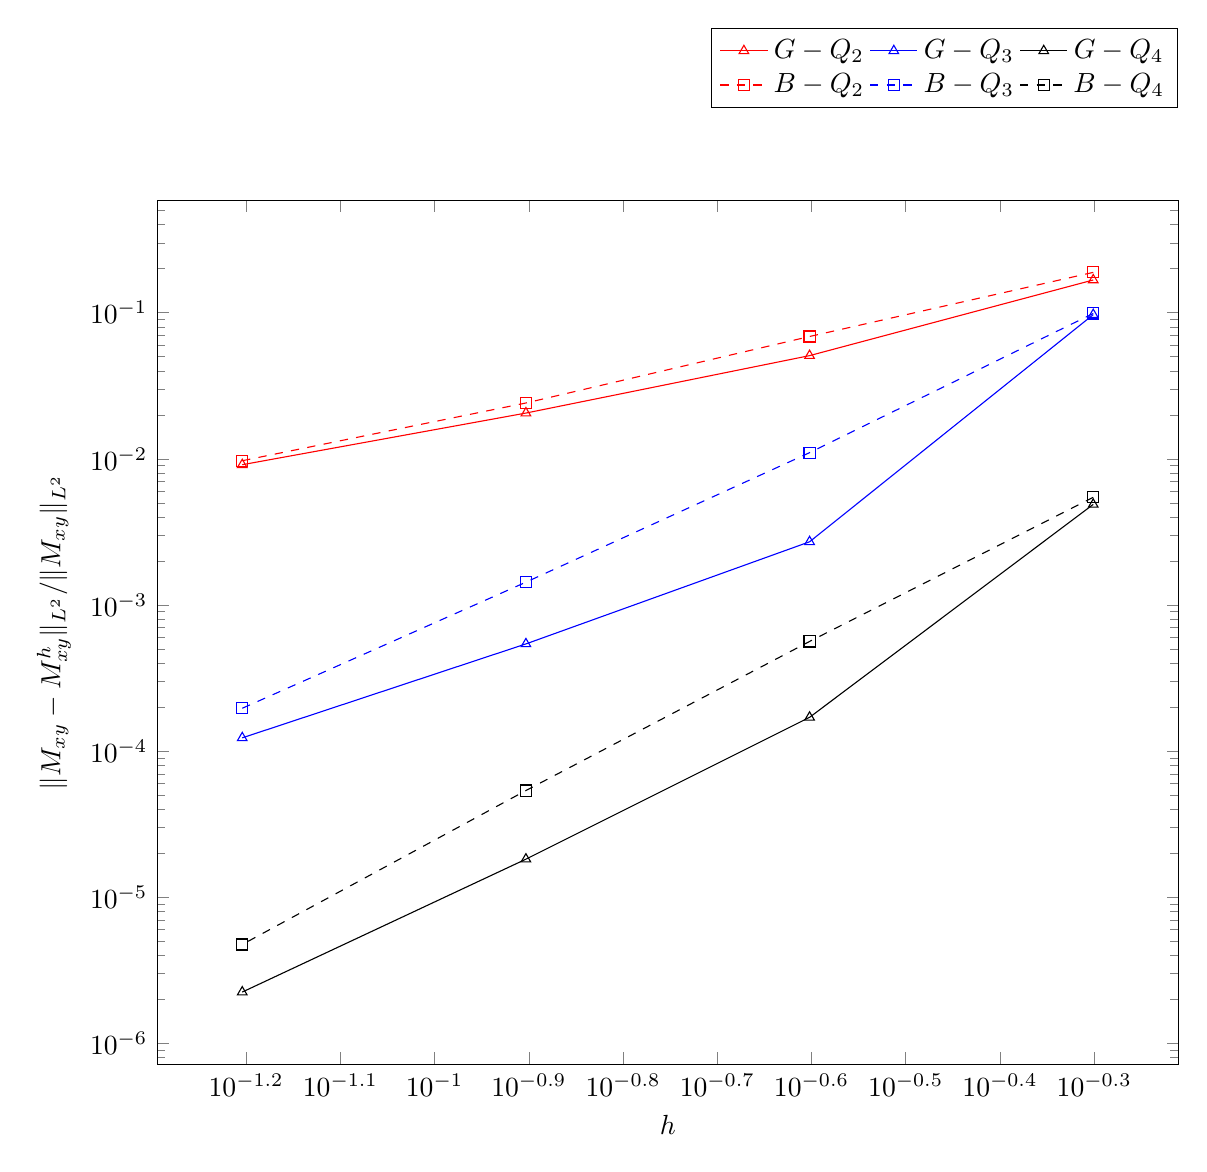
\begin{tikzpicture}
    \begin{loglogaxis}[
        legend columns=3,
    	legend style={at={(1,1.2)}, nodes={scale=1, transform shape}},
        xlabel=$h$,
        ylabel=${\|M_{xy}-M_{xy}^{h}\|_{L^2}}/{\|M_{xy}\|_{L^2}}$ ,
        width=1.2\textwidth
    ]

    \addplot [color=red,mark=triangle] plot coordinates {

        (.5,       0.167365)
        (.25,       0.0508268)
        (.125,      0.020567)
        (.0625,     0.0091148)
    };

    
    \addplot [color=blue,mark=triangle] plot coordinates {

        (.5,        0.0969531)
        (.25,       0.0027069)
        (.125,      0.000541529)
        (.0625,     0.000123283)
    };

    \addplot [color=black,mark=triangle] plot coordinates {

        (.5,        0.00487662)
        (.25,       0.000170379)
        (.125,      1.82393e-05)
        (.0625,     2.24704e-06)
    };

    \addplot [color=red,mark=square, every mark/.append style={solid}, dashed] plot coordinates {

        (.5,        0.188695)
        (.25,       0.0687081)
        (.125,      0.0241024)
        (.0625,     0.0097052)
    };

    
    \addplot [color=blue,mark=square, every mark/.append style={solid}, dashed] plot coordinates {

        (.5,        0.0987883)
        (.25,       0.0110221)
        (.125,      0.00143233)
        (.0625,     0.000196494)
    };

    \addplot [color=black,mark=square, every mark/.append style={solid}, dashed] plot coordinates {

        (.5,        0.00545265)
        (.25,       0.000562985)
        (.125,      5.37704e-05)
        (.0625,     4.7544e-06)
    };

    \logLogSlopeTriangle{0.25}{0.17}{0.07}{3}{black};
    \logLogSlopeTriangle{0.25}{0.17}{0.36}{2}{blue};
    \logLogSlopeTriangle{0.25}{0.17}{0.68}{1}{red};

    \legend{$G-Q_2$\\$G-Q_3$\\$G-Q_4$\\$B-Q_2$\\$B-Q_3$\\$B-Q_4$\\}
    \end{loglogaxis}
\end{tikzpicture}

\end{document}
